\documentclass[11pt]{article}
\usepackage[margin=1in]{geometry}

\usepackage{amsmath}
\usepackage{amssymb}
\usepackage[utf8]{inputenc} 
\usepackage{graphicx} 
\usepackage{parskip} 
\usepackage{multirow} 
\usepackage{mathtools}

\DeclarePairedDelimiter\abs{\lvert}{\rvert}%
\DeclarePairedDelimiter\norm{\lVert}{\rVert}%

\makeatletter
\let\oldabs\abs
\def\abs{\@ifstar{\oldabs}{\oldabs*}}

\let\oldnorm\norm
\def\norm{\@ifstar{\oldnorm}{\oldnorm*}}
\makeatother
\usepackage{multicol} 
\usepackage[spanish,es-nodecimaldot]{babel} 
\usepackage{mathtools}
\usepackage{amsfonts}
\usepackage{float}
\usepackage{textcomp}
\usepackage{caption}
\usepackage{subfig}
\usepackage[spanish]{babel}
\usepackage{gensymb}
\def\sen{\mathop{\mbox{\normalfont sen}}\nolimits}

\usepackage{fancyhdr}
\fancyhf{}
\rfoot{\thepage}
\pagestyle{fancy}
\lhead{Nieto Castellanos Jaime Fabián}
\chead{}
\rhead{Tarea 4. Histogramas}
\begin{document}


\textbf{Inciso 3)}
\begin{figure}[H]
\centering
\subfloat[\centering En la figura del lado izquierdo se muestra el histograma para todos los PMT, mientras que en la del lado derecho únicamente para los cuarenta primeros PMT usados.]{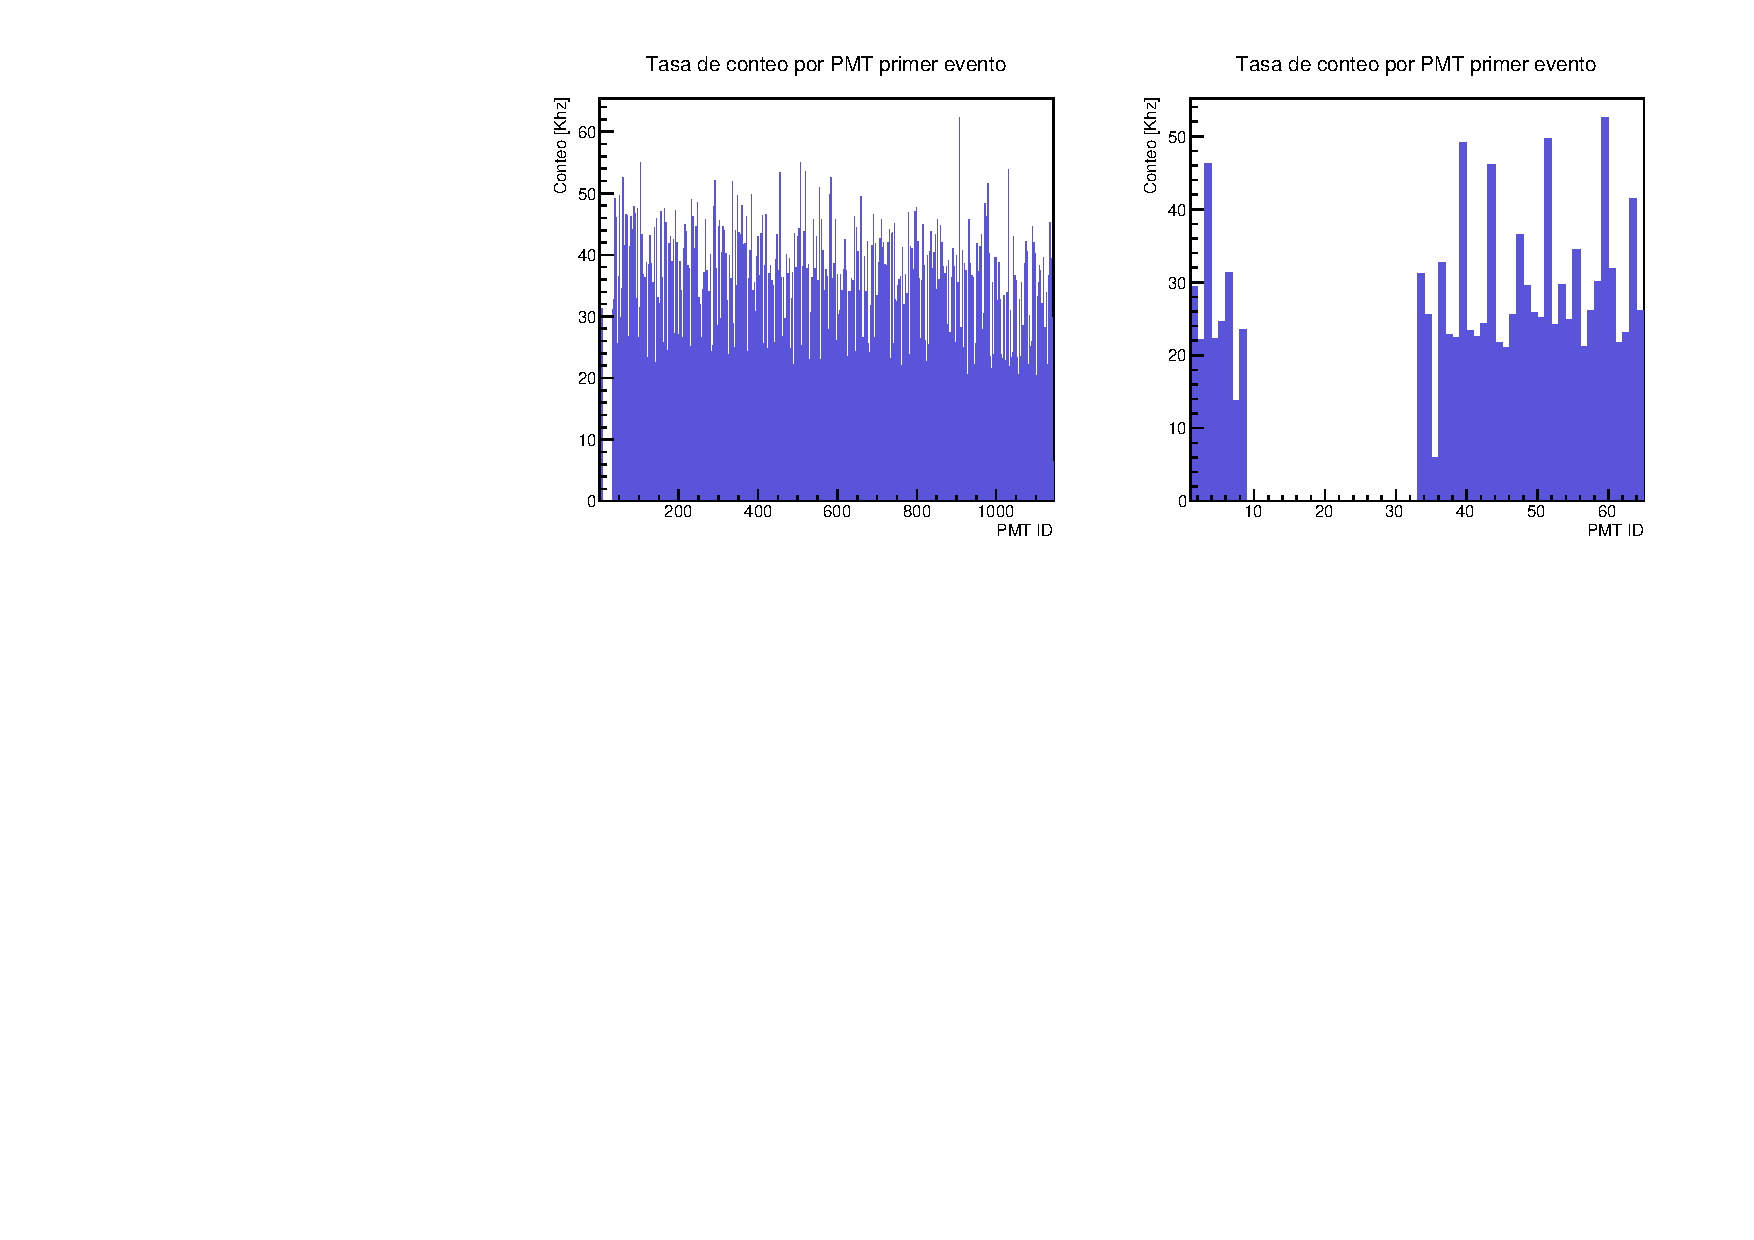
\includegraphics[width=1\textwidth]{../Figuras/Prob3PrimerEvento.pdf}}

\subfloat[\centering En la figura del lado izquierdo se muestra el histograma para todos los PMT, mientras que en la del lado derecho únicamente para los cuarenta primeros PMT usados.]{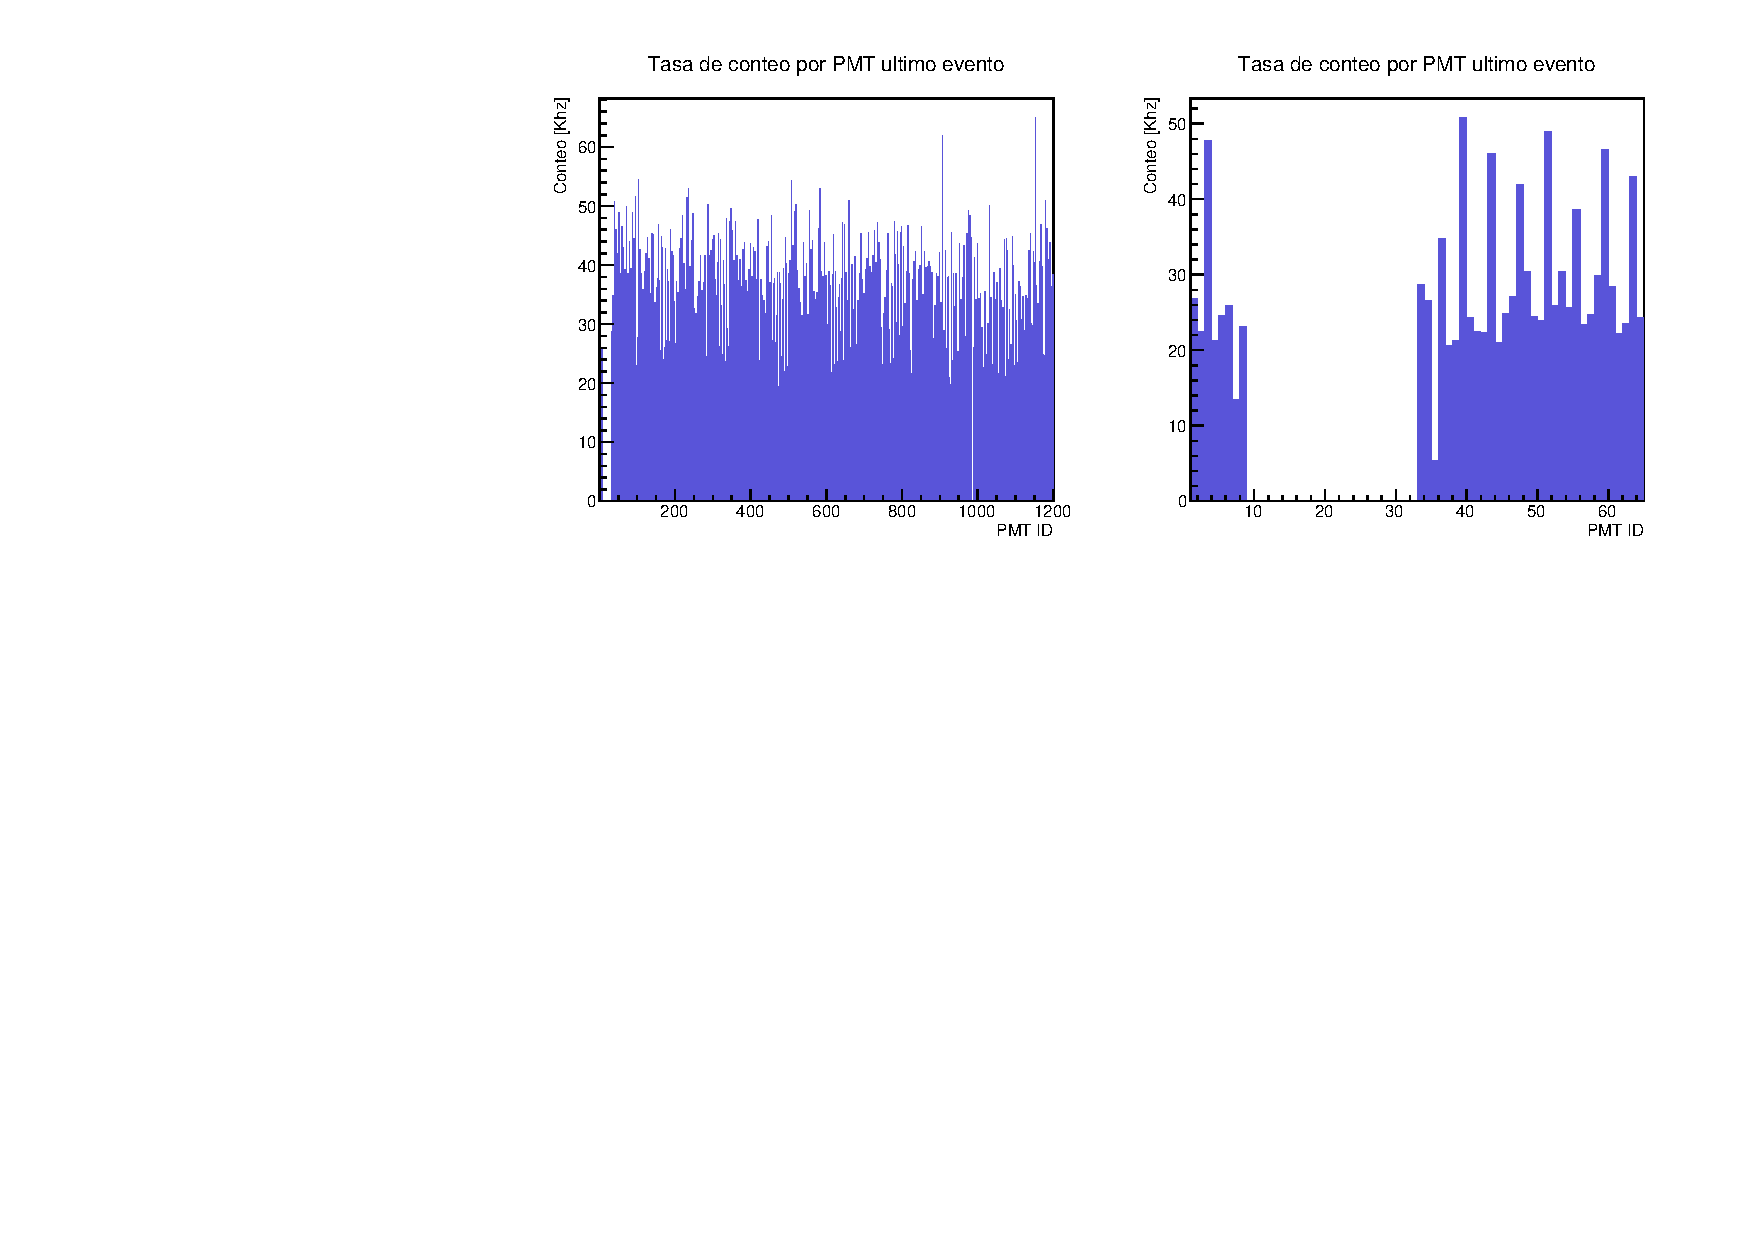
\includegraphics[width=1\textwidth]{../Figuras/Prob3UltimoEvento.pdf}}
\caption{Histogramas en donde se muestra la tasa de conteo en kHz de cada PMT para el evento 0 (a) y el último evento (b).}
\label{fig:Prob3}
\end{figure}
\pagebreak

\textbf{Inciso 4)}

\begin{figure}[H]
\centering
\subfloat[\centering En la figura del lado izquierdo se muestra el histograma para todos los tanques, mientras que en la del lado derecho únicamente para los cuarenta primeros tanques usados.]{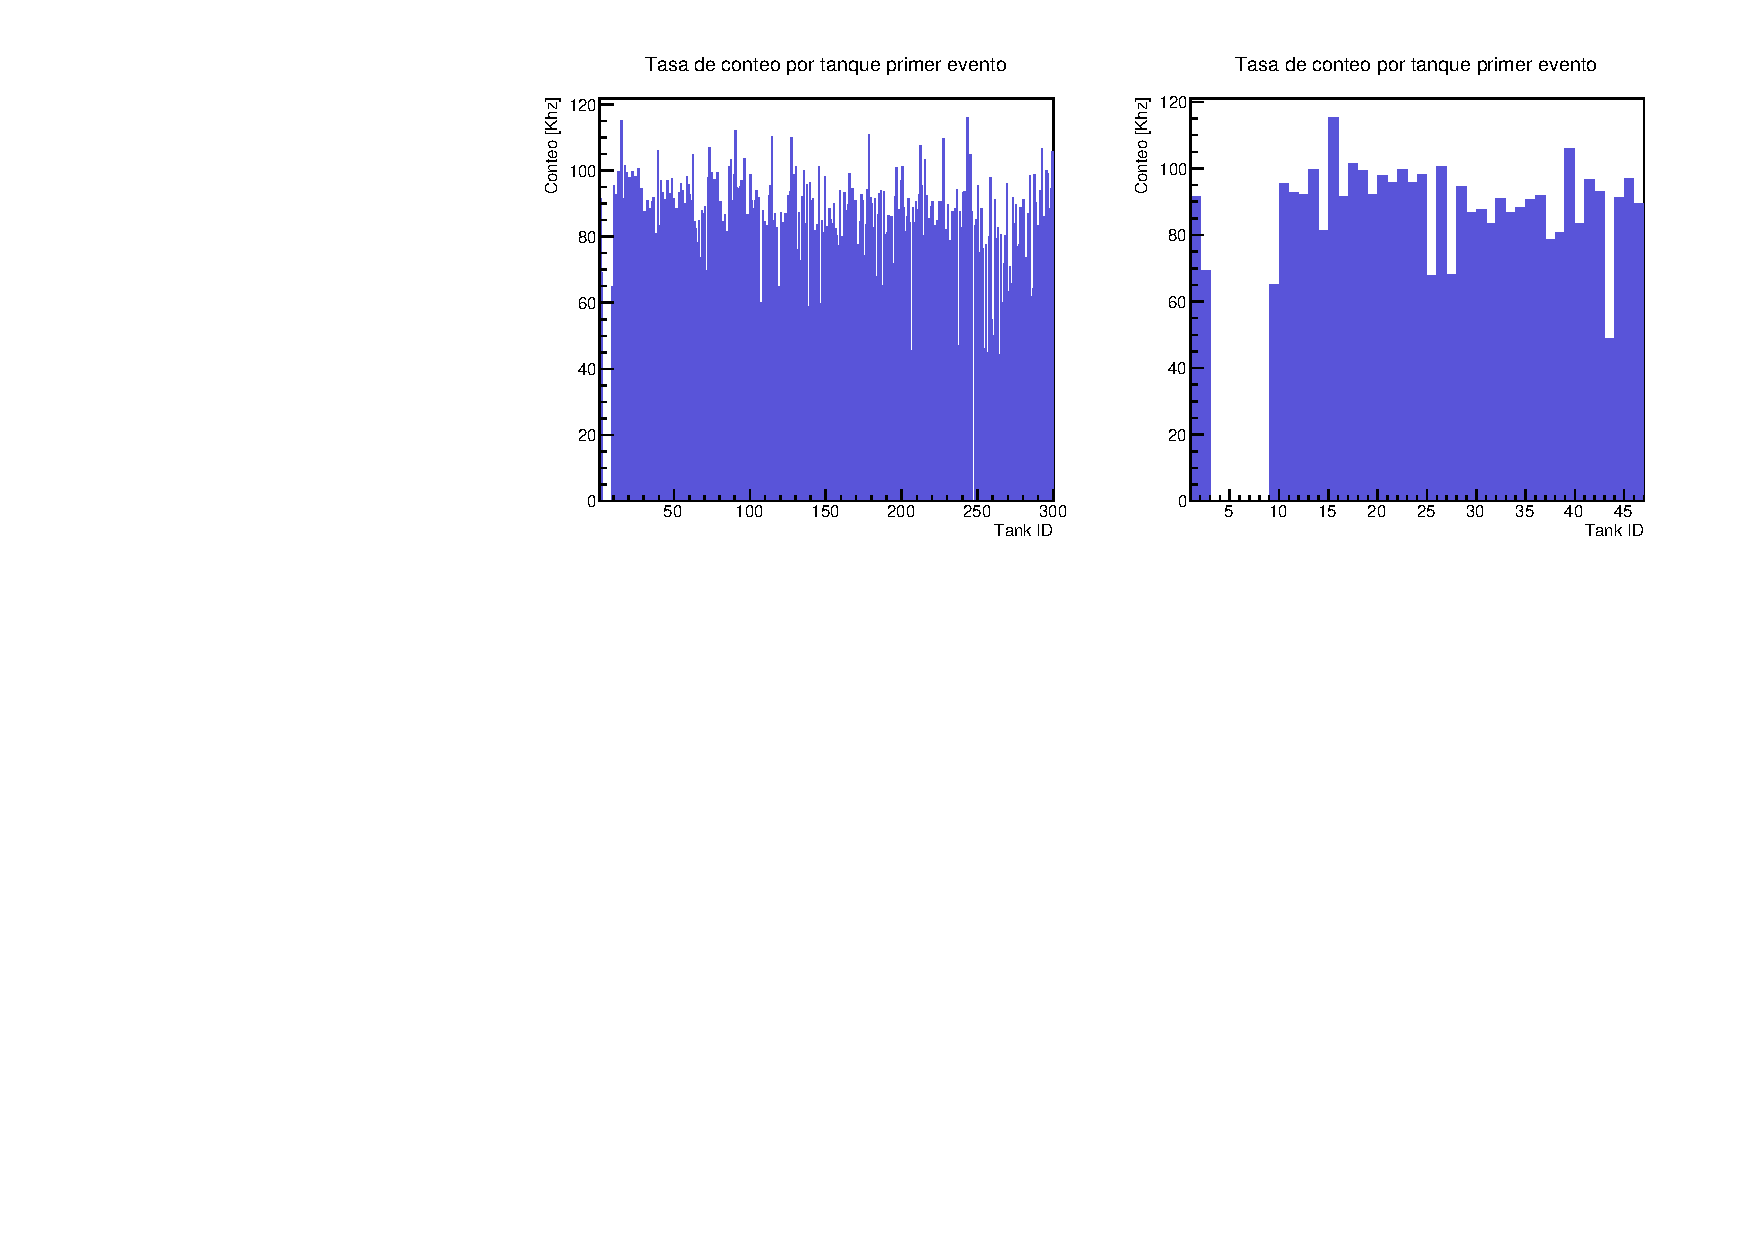
\includegraphics[width=1\textwidth]{../Figuras/Prob4PrimerEvento.pdf}}

\subfloat[\centering En la figura del lado izquierdo se muestra el histograma para todos los tanques, mientras que en la del lado derecho únicamente para los cuarenta primeros tanques usados.]{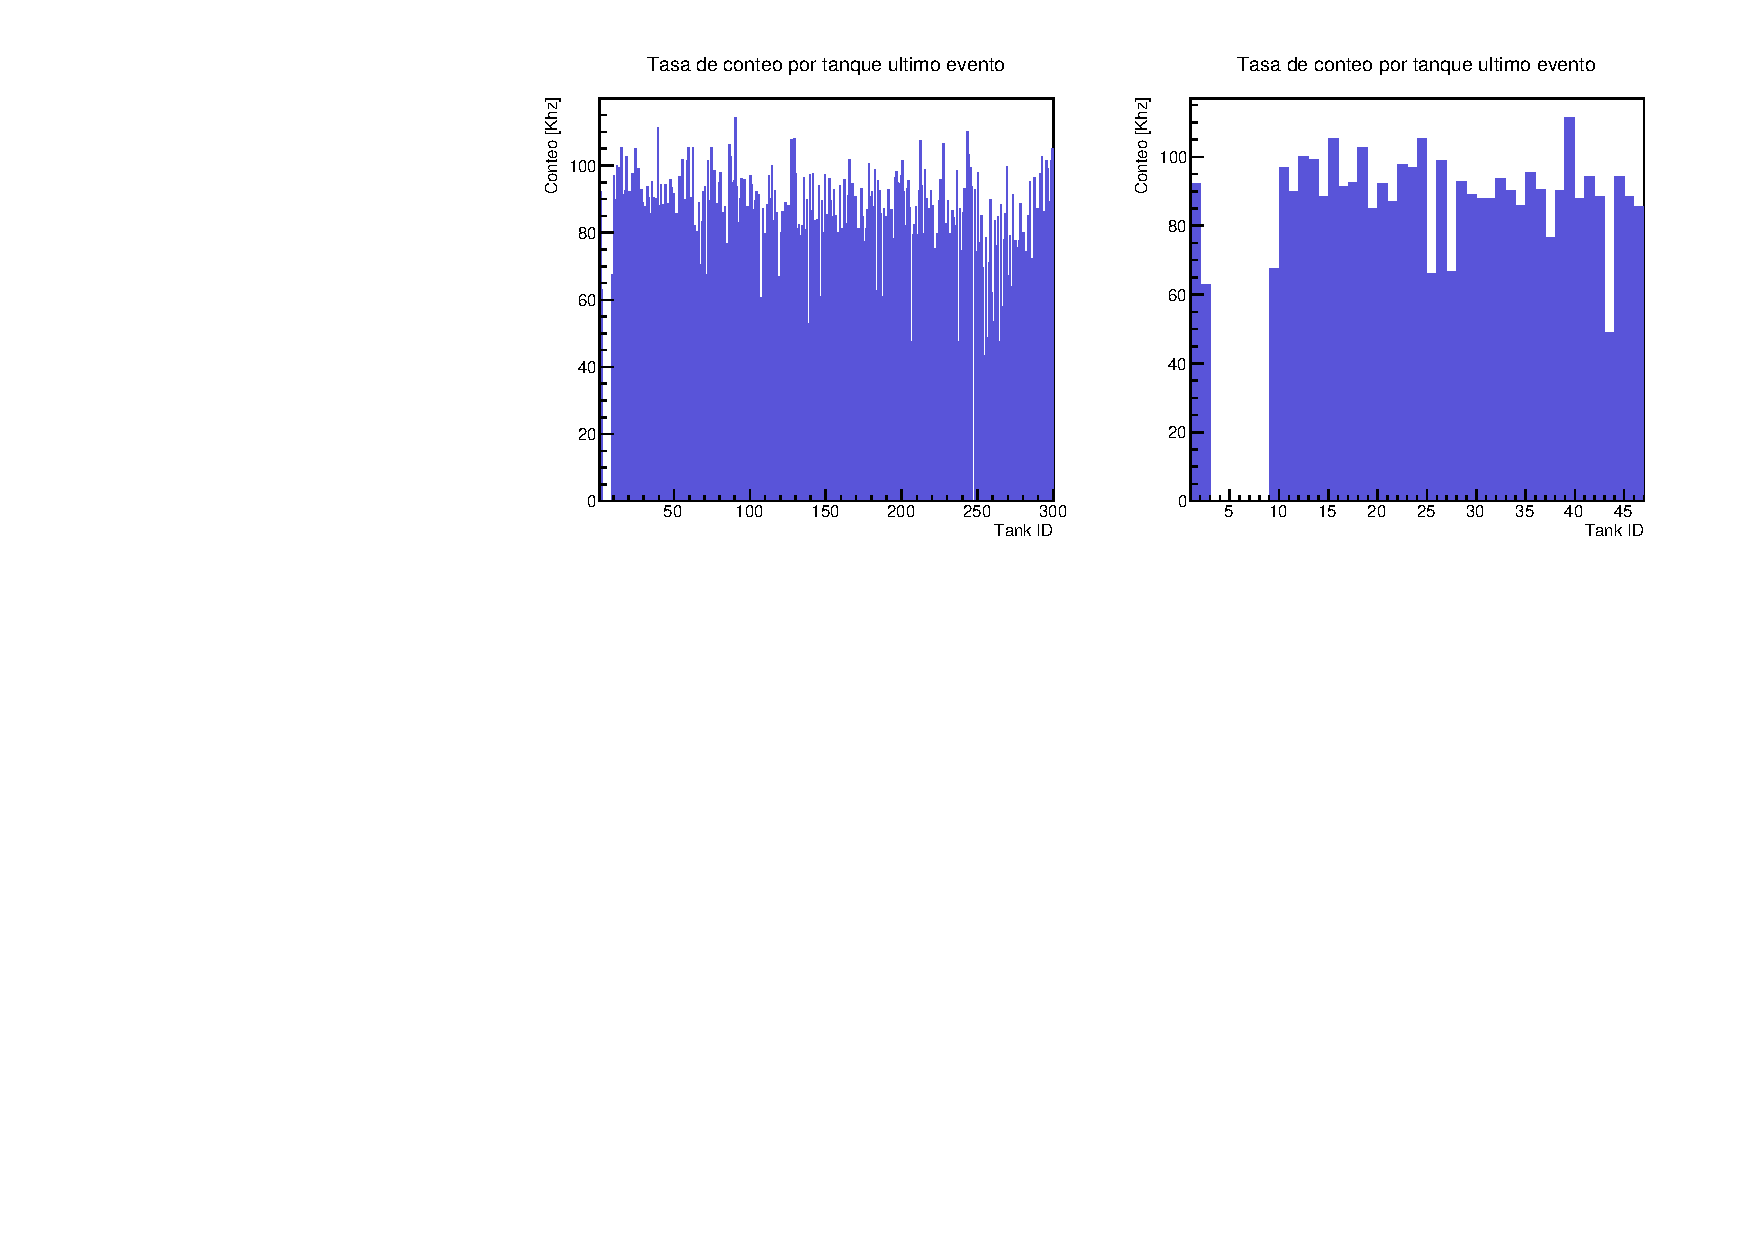
\includegraphics[width=1\textwidth]{../Figuras/Prob4UltimoEvento.pdf}}
\caption{Histogramas en donde se muestra la tasa de conteo en kHz de cada tanque para el evento 0 (a) y el último evento (b).}
\label{fig:Prob4}
\end{figure}

\textbf{Inciso 5)}

\begin{figure}[H]
\centering
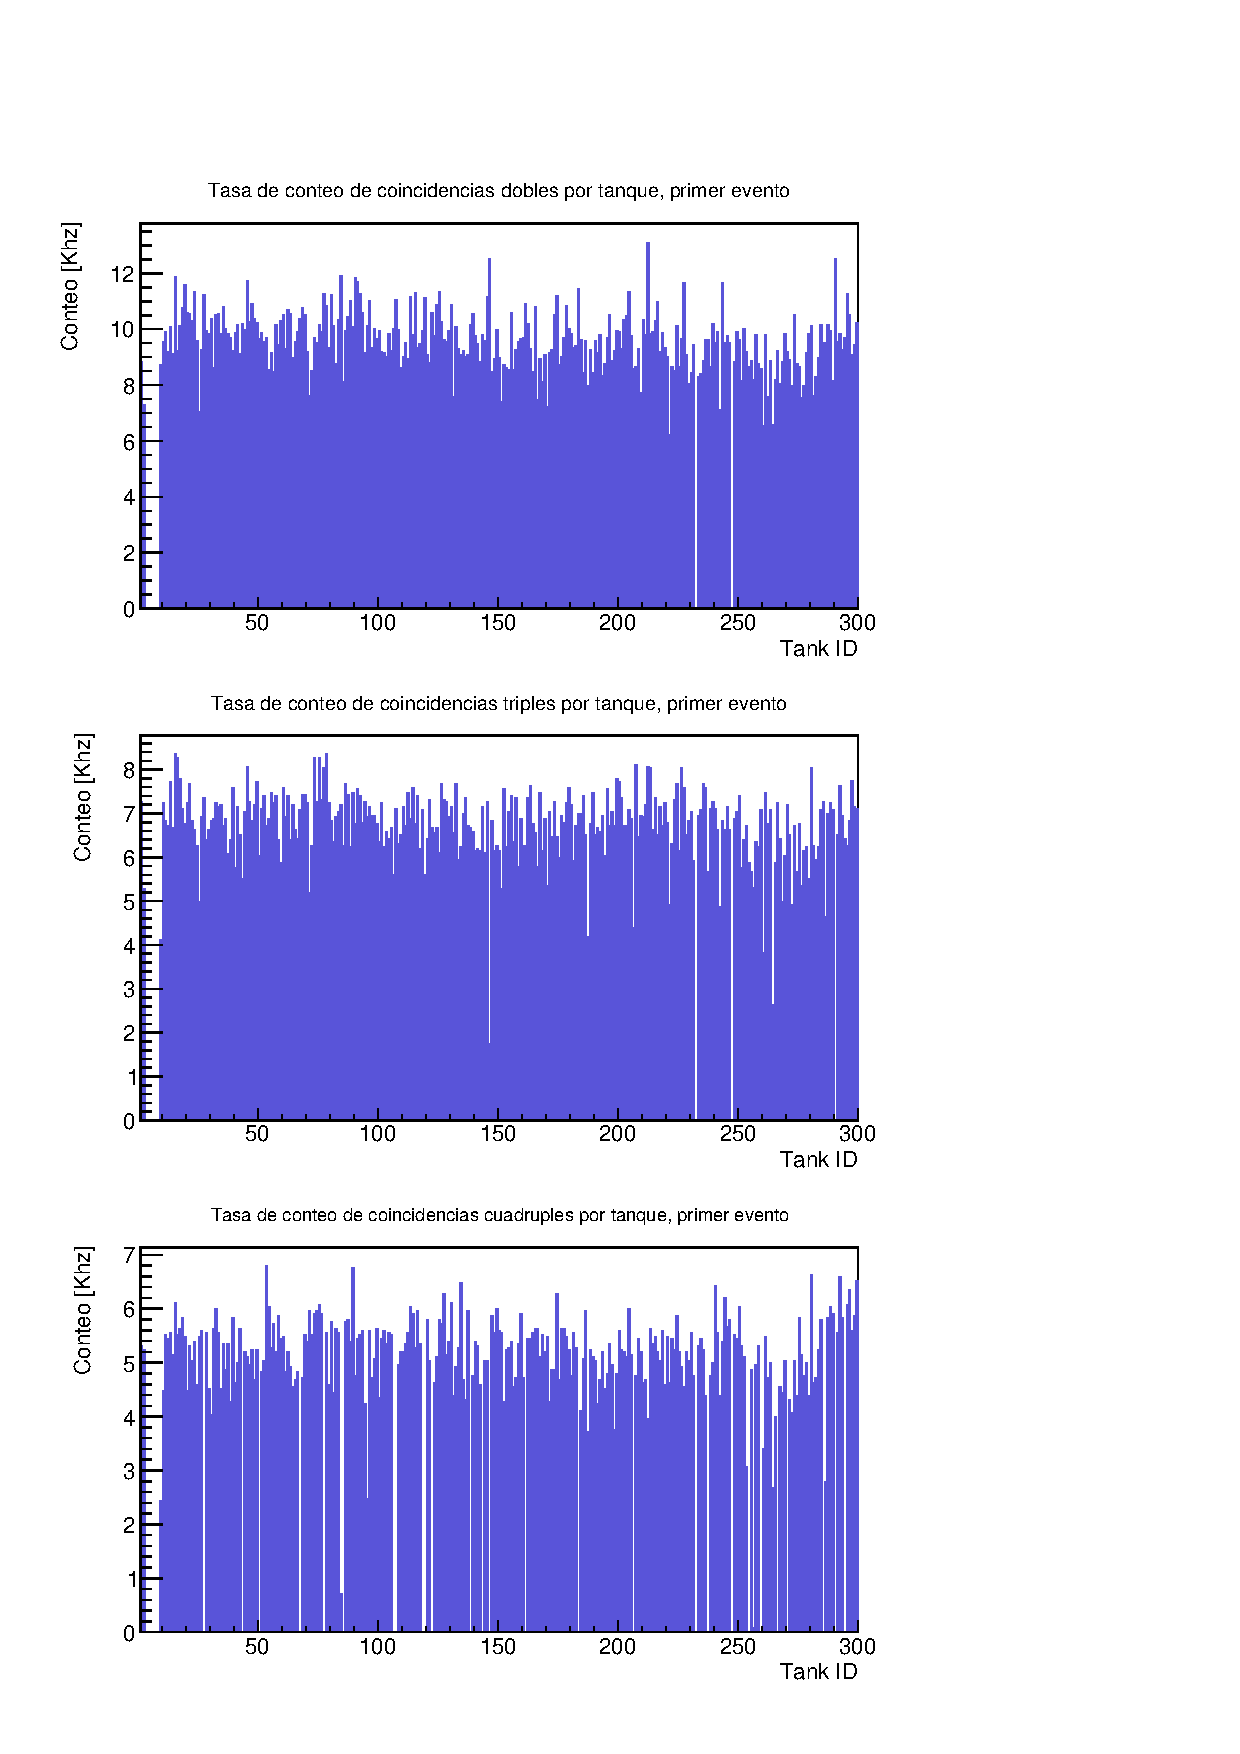
\includegraphics[width=0.8 \textwidth]{../Figuras/Prob5PrimerEvento.pdf}
\caption{Tasas de conteo de coincidencias para el primer evento. De arribo a abajo se van mostrando los resultados para coincidencias dobles, triples y cuádruples.}
\label{fig:Prob5-1}
\end{figure}


\begin{figure}[H]
\centering
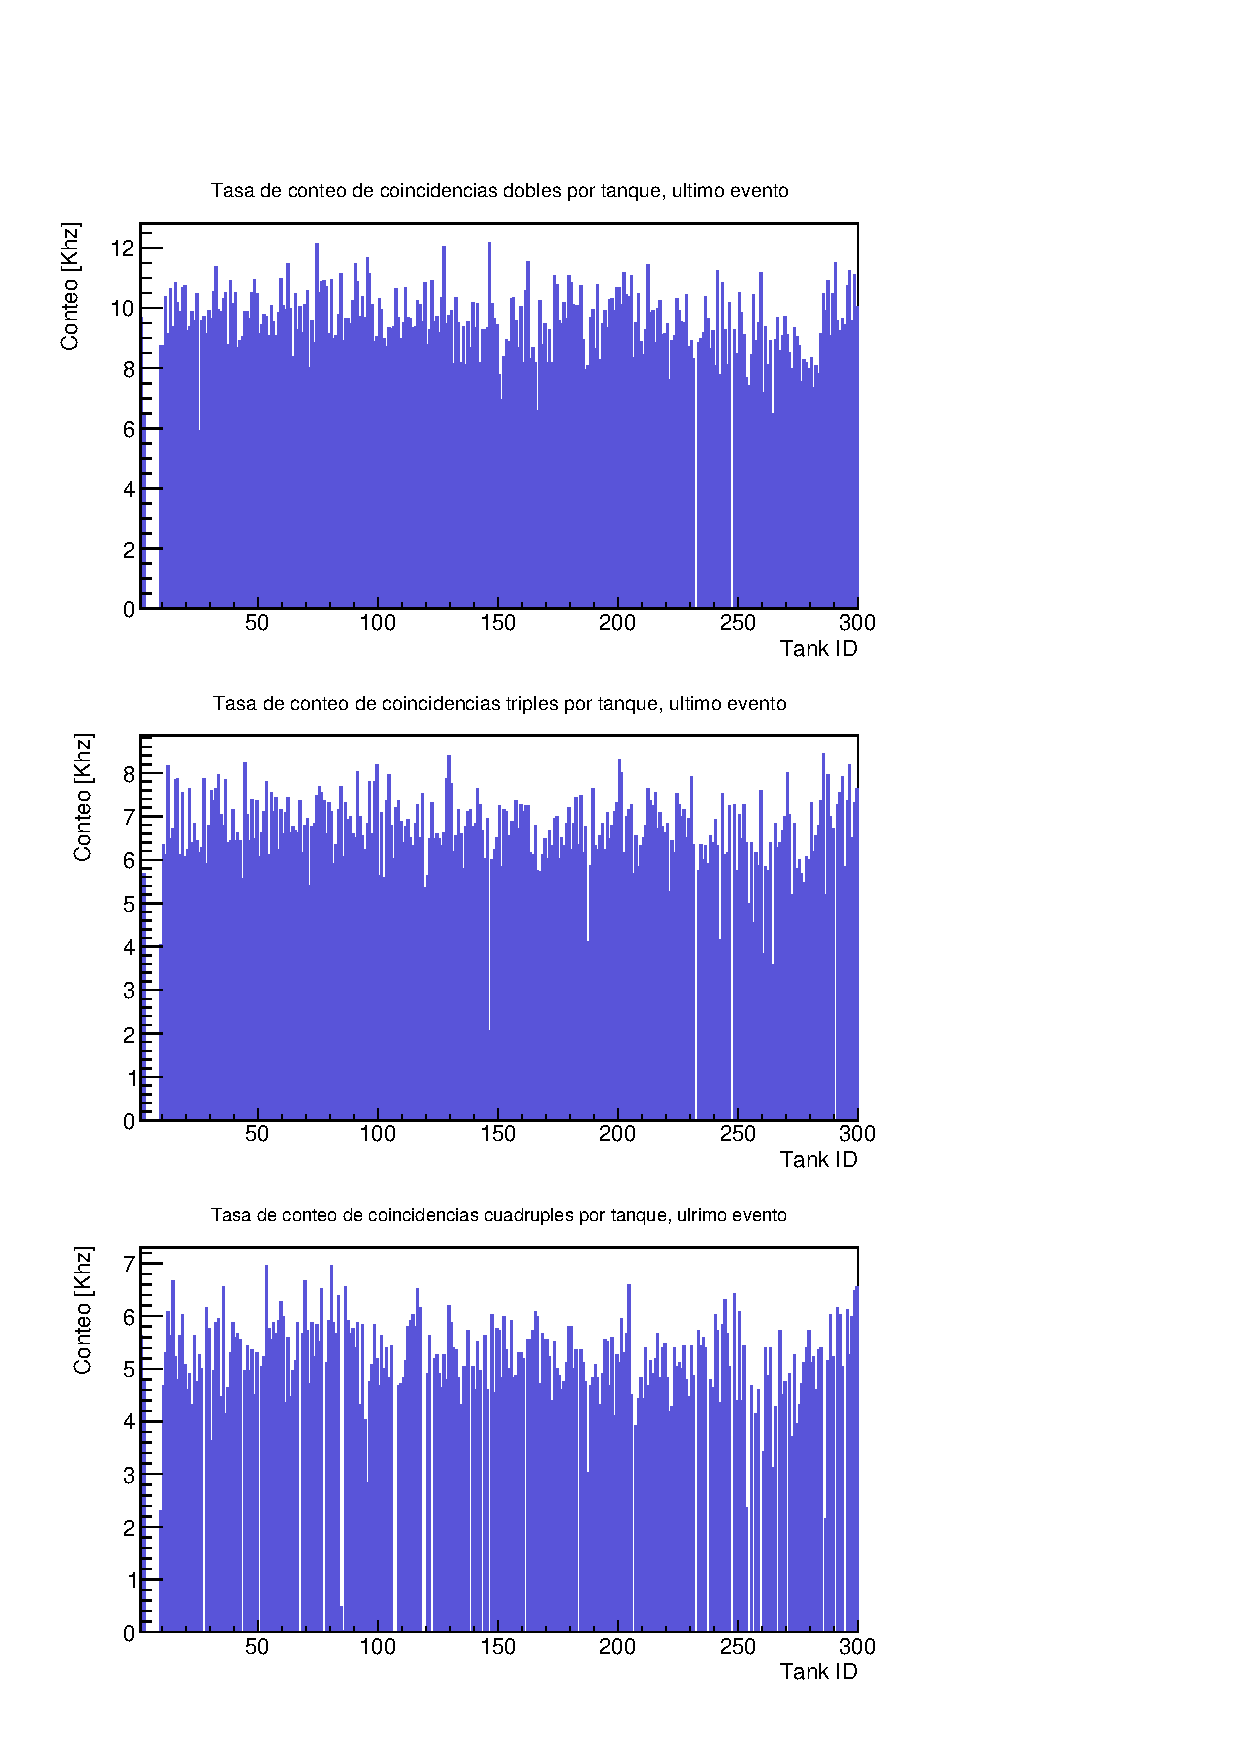
\includegraphics[width=0.8\textwidth]{../Figuras/Prob5UltimoEvento.pdf}
\caption{Tasas de conteo de coincidencias para el último evento. De arribo a abajo se van mostrando los resultados para coincidencias dobles, triples y cuádruples.}
\label{fig:Prob5-2}
\end{figure}


\textbf{Inciso 6)}


\begin{figure}[H]
\centering
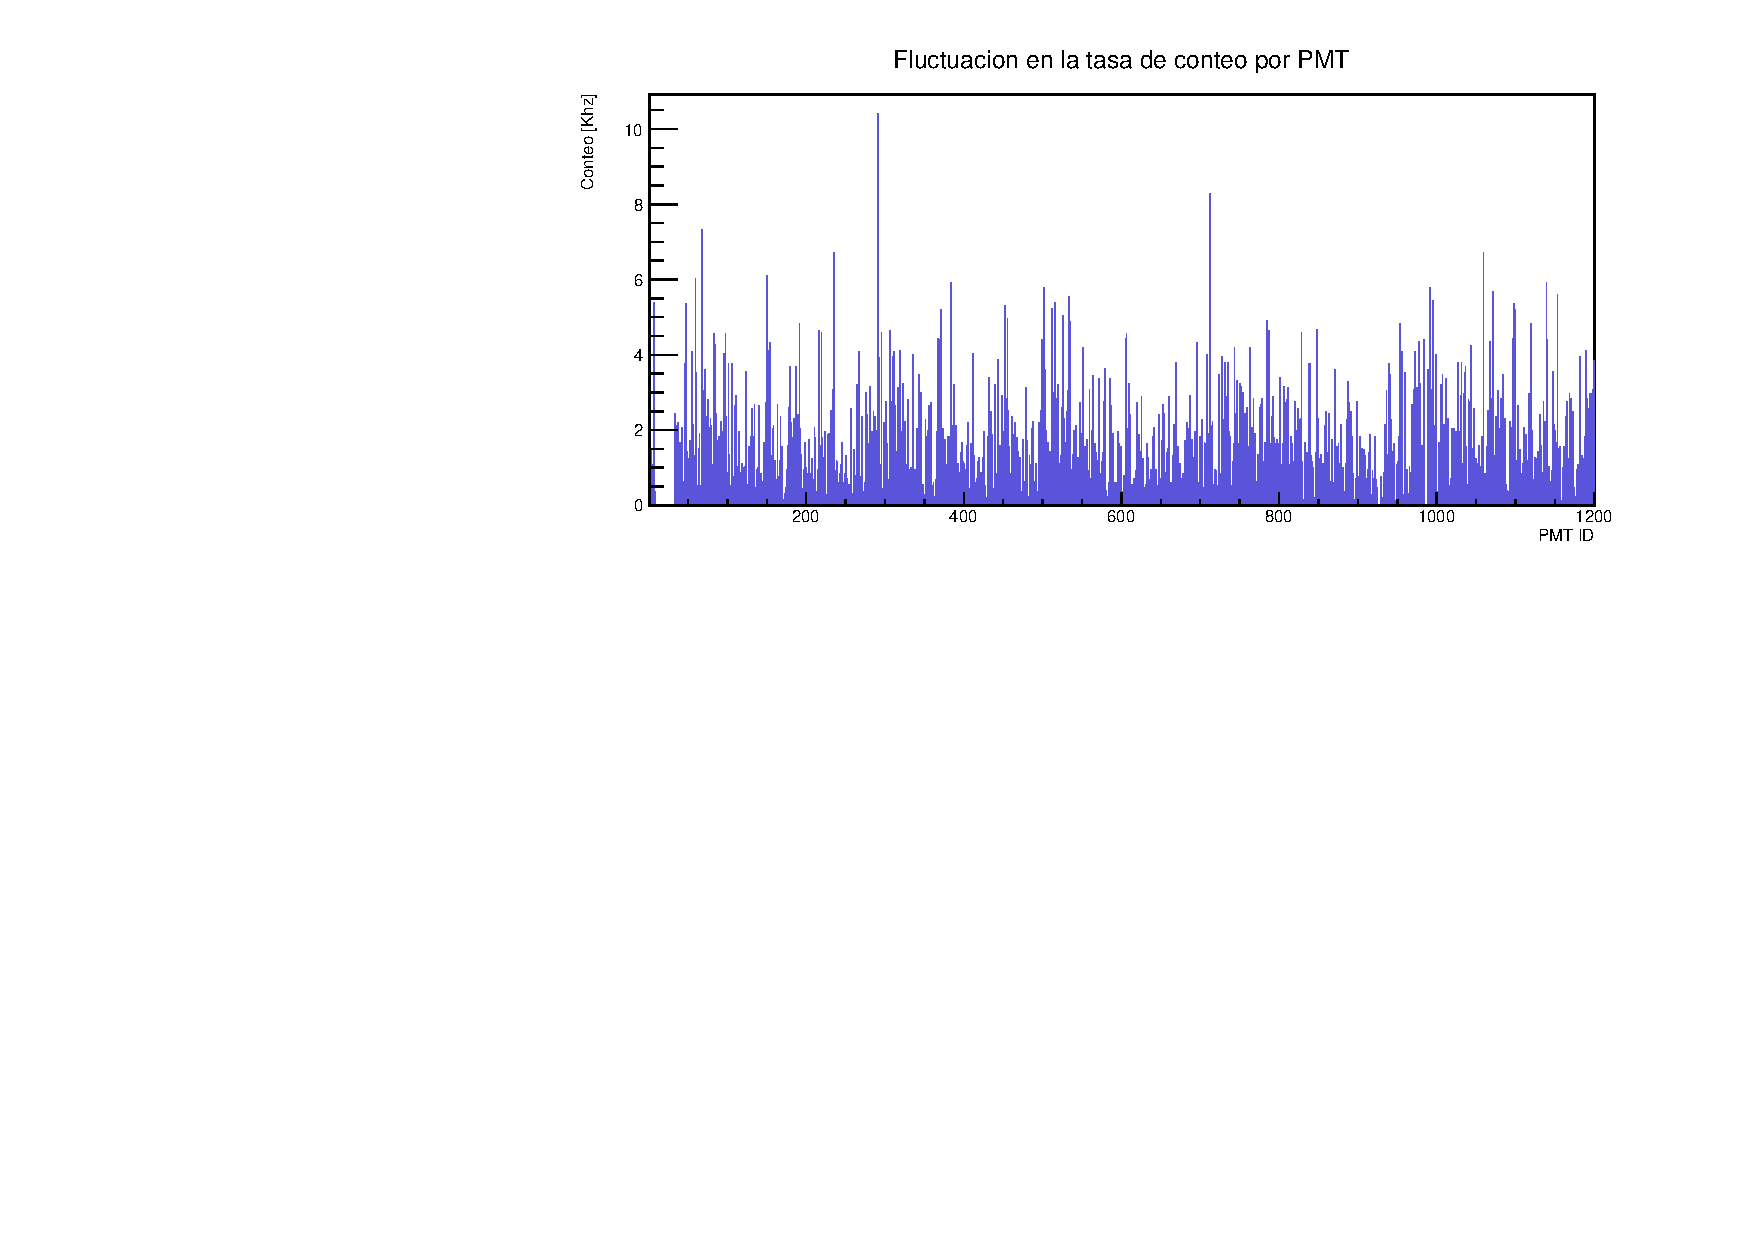
\includegraphics[width=1\textwidth]{../Figuras/Fluctuaciones.pdf}
\caption{Fluctuación de la tasa de conteo de los PMT. Se restaron los histogramas mostrados en el inciso 3).}
\label{fig:Prob6}
\end{figure}

Se observa que en la mayoría de los casos las fluctuaciones se encuentran por debajo de 4 kHz, que es un orden de magnitud menor al de las tasa de fluctuaciones, las cuales son del orden de 10 kHz. Sólo hay una situación en la que hay una excepción, en el cual se aprecia un pico que está por arriba de 10 kHz entre el PMT de ID 200 y el de ID 400. En dicho caso posiblemente lo que sucedió es que en el primer o último evento, no se usó un PMT que en el otro evento sí se ocupó y por lo tanto al restar los histogramas obtenemos un pico que sobresale. 

\textbf{Inciso 7)}


\begin{figure}[H]
\centering
\subfloat[\centering Coincidencias dobles para diferentes subruns, primer evento.]{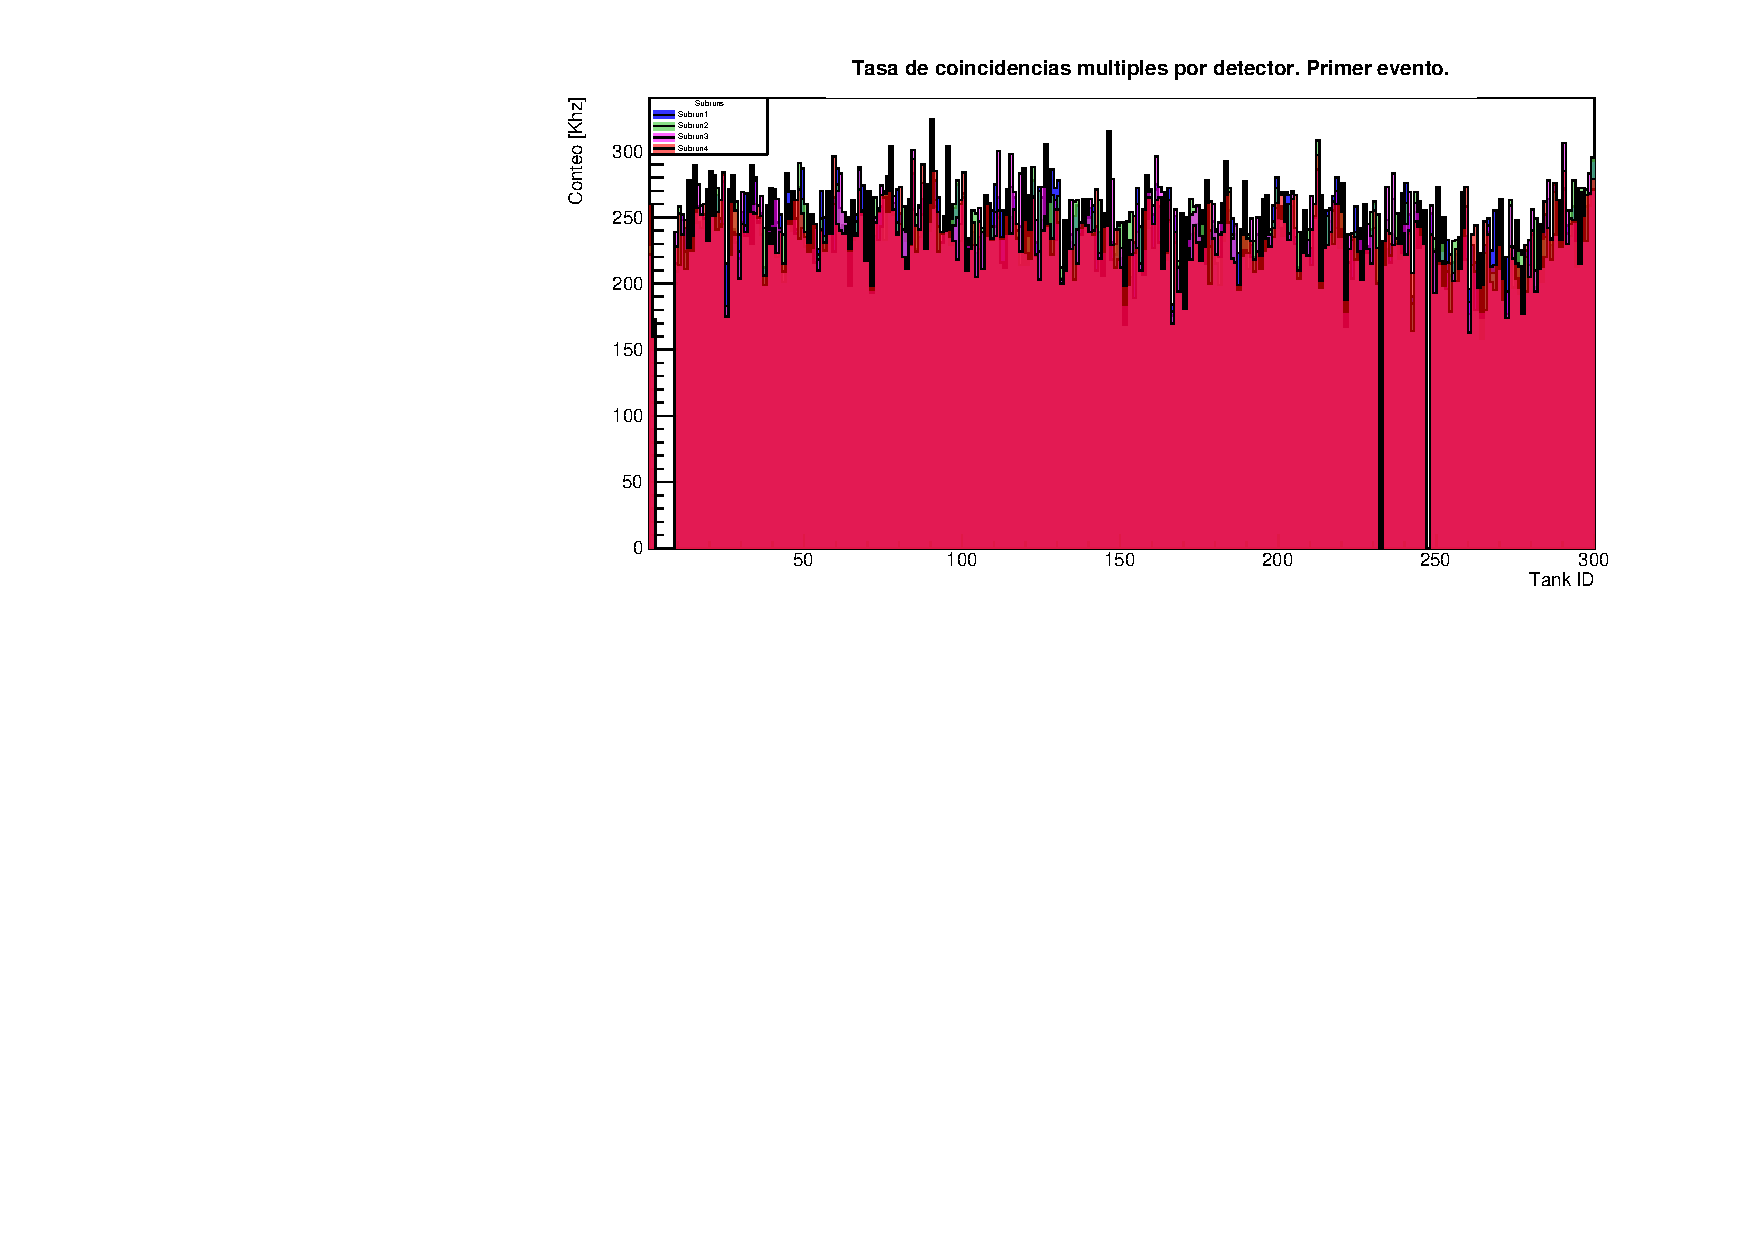
\includegraphics[width=0.9\textwidth]{../Figuras/CoinDoblesSubruns.pdf}}
\end{figure}

\begin{figure}[H]
\centering
\subfloat[\centering Coincidencias triples para diferentes subruns, primer evento.]{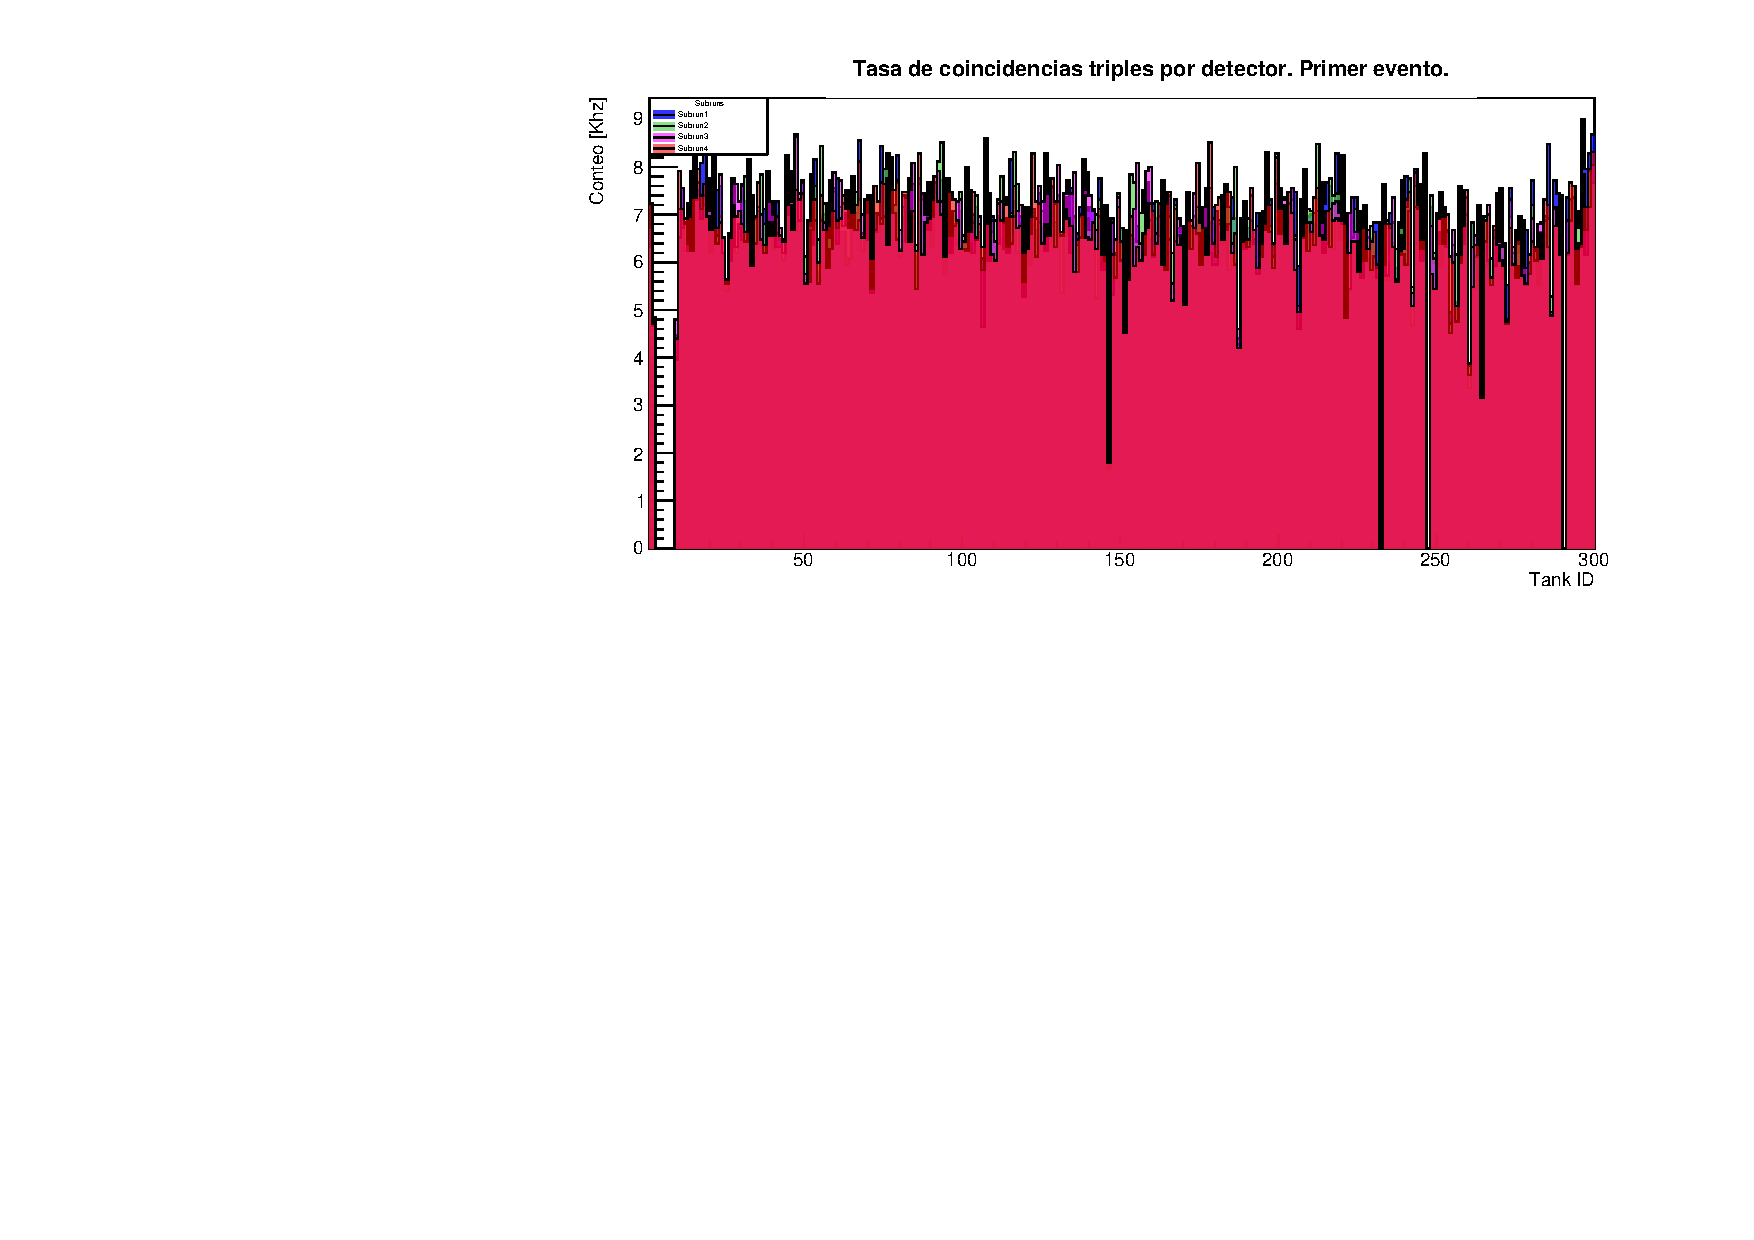
\includegraphics[width=0.9\textwidth]{../Figuras/CoinTriplesSubruns.pdf}}

\subfloat[\centering Coincidencias cuádruples para diferentes subruns, primer evento.]{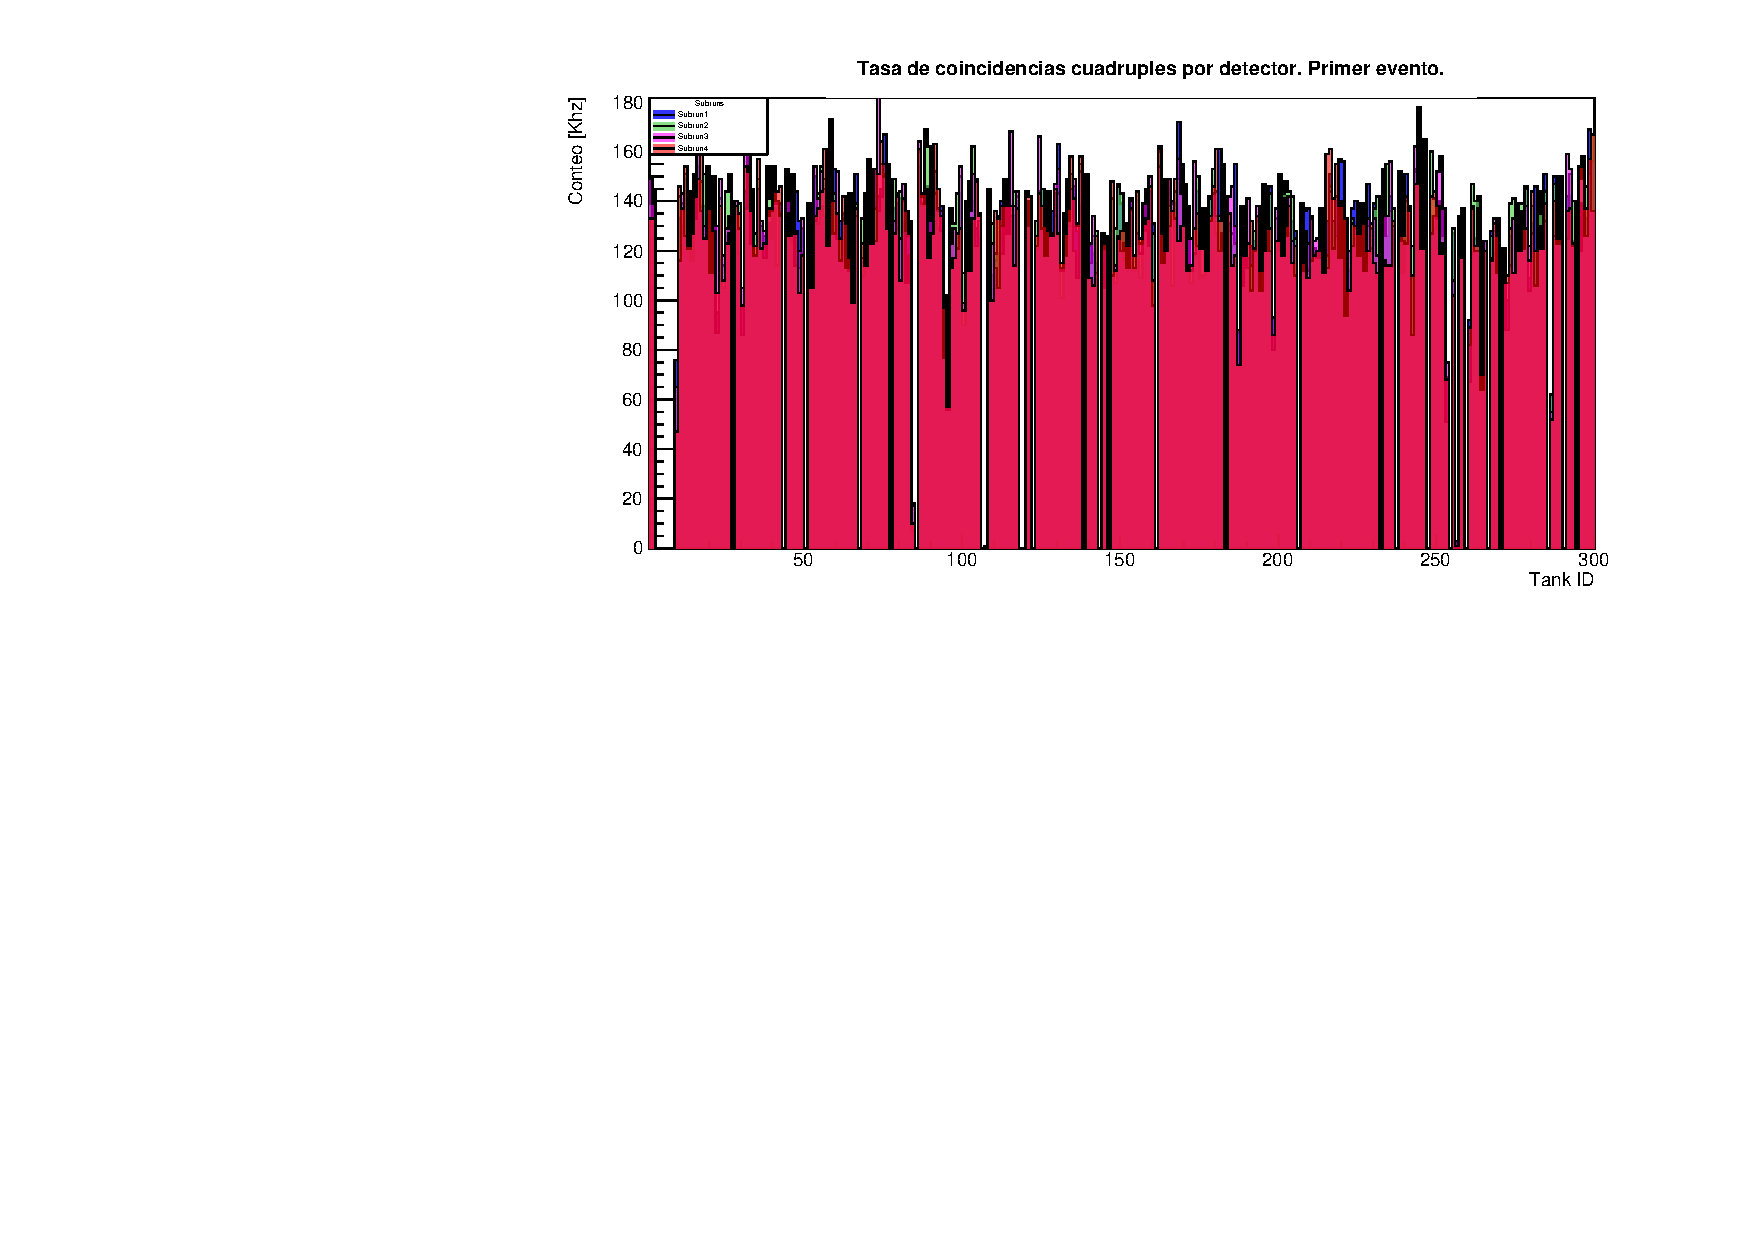
\includegraphics[width=0.9\textwidth]{../Figuras/CoinCuadruplesSubruns.pdf}}
\caption{Tasas de conteo de coincidencias para el primer evento usando diferentes subruns. De arribo a abajo se van mostrando los resultados para coincidencias dobles, triples y cuádruples.}
\label{fig:Prob7-1}
\end{figure}

\begin{figure}[H]
\centering
\subfloat[\centering Coincidencias dobles para diferentes subruns, último evento.]{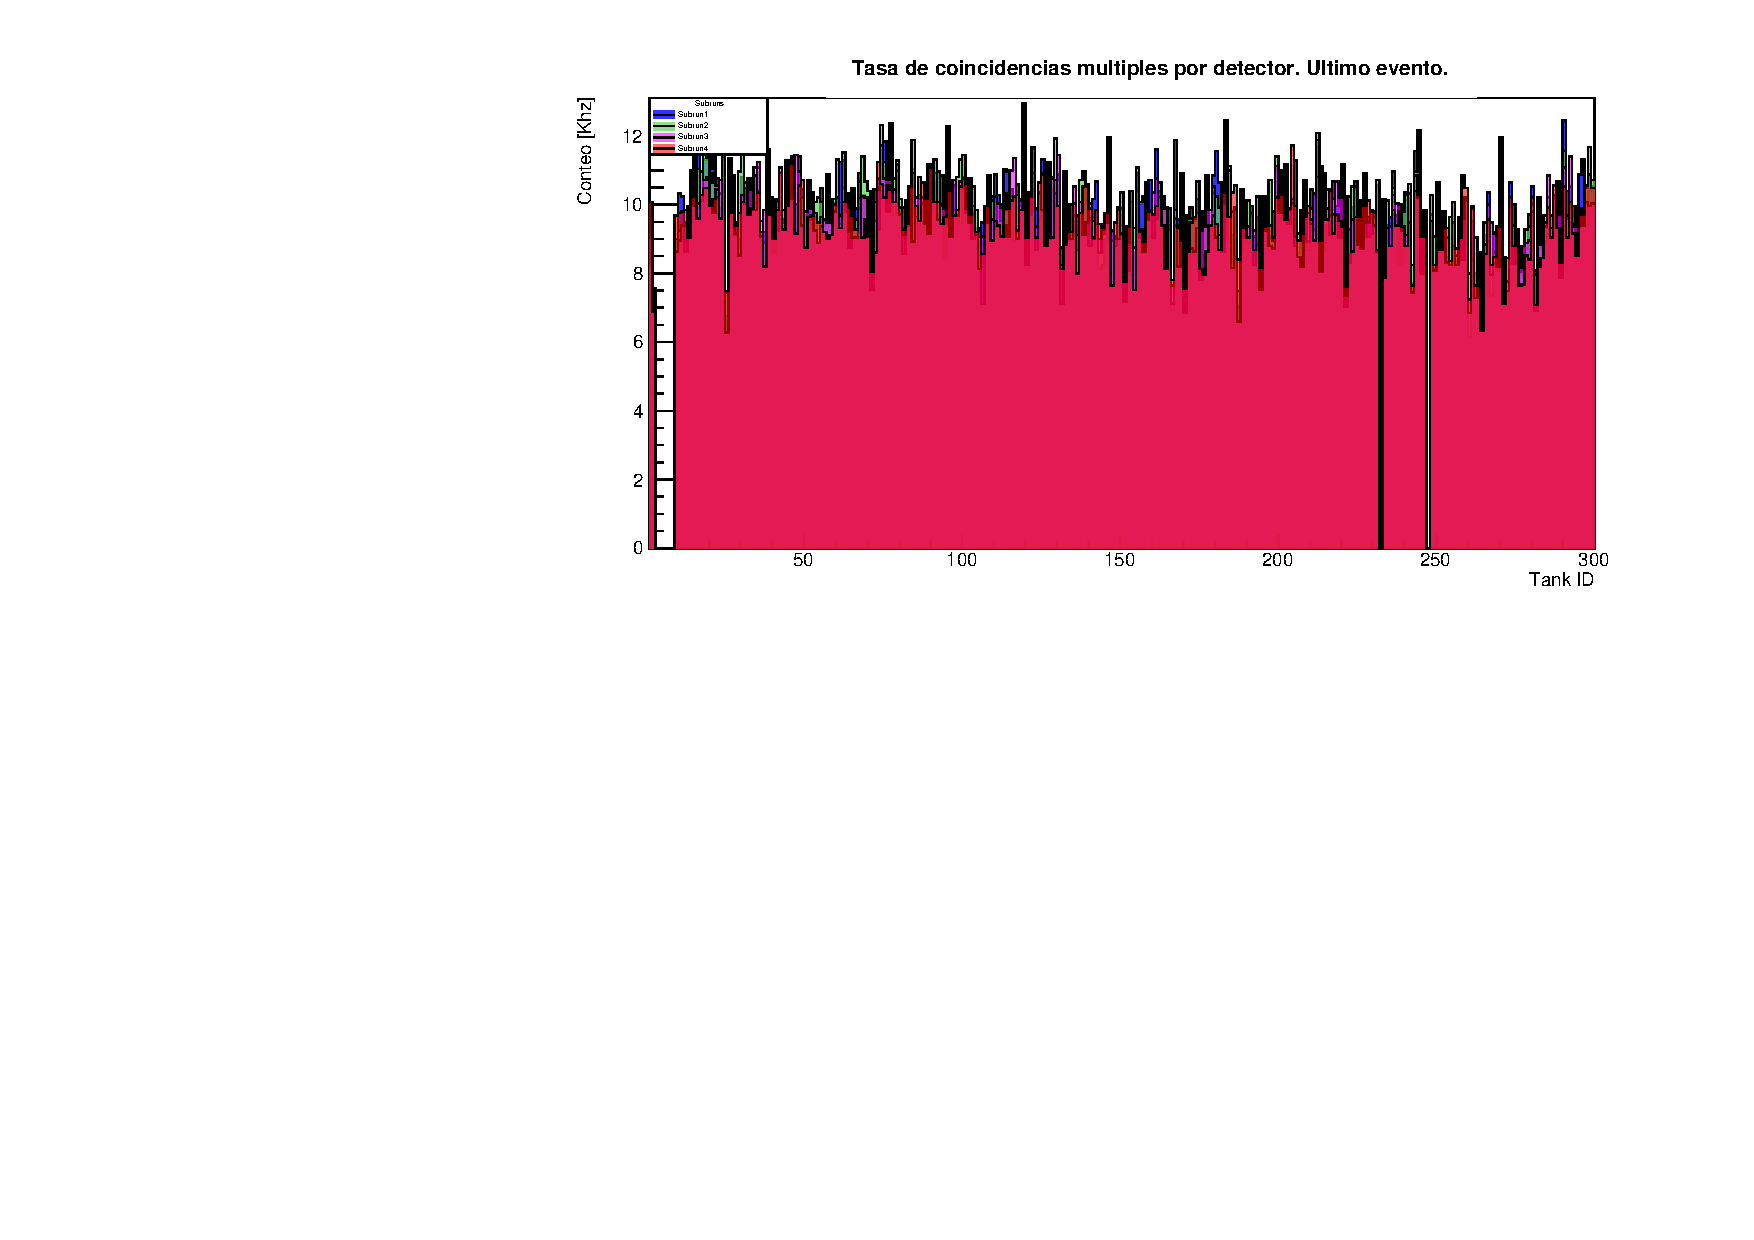
\includegraphics[width=0.9\textwidth]{../Figuras/CoinDoblesSubrunsUE.pdf}}

\subfloat[\centering Coincidencias triples para diferentes subruns, último evento.]{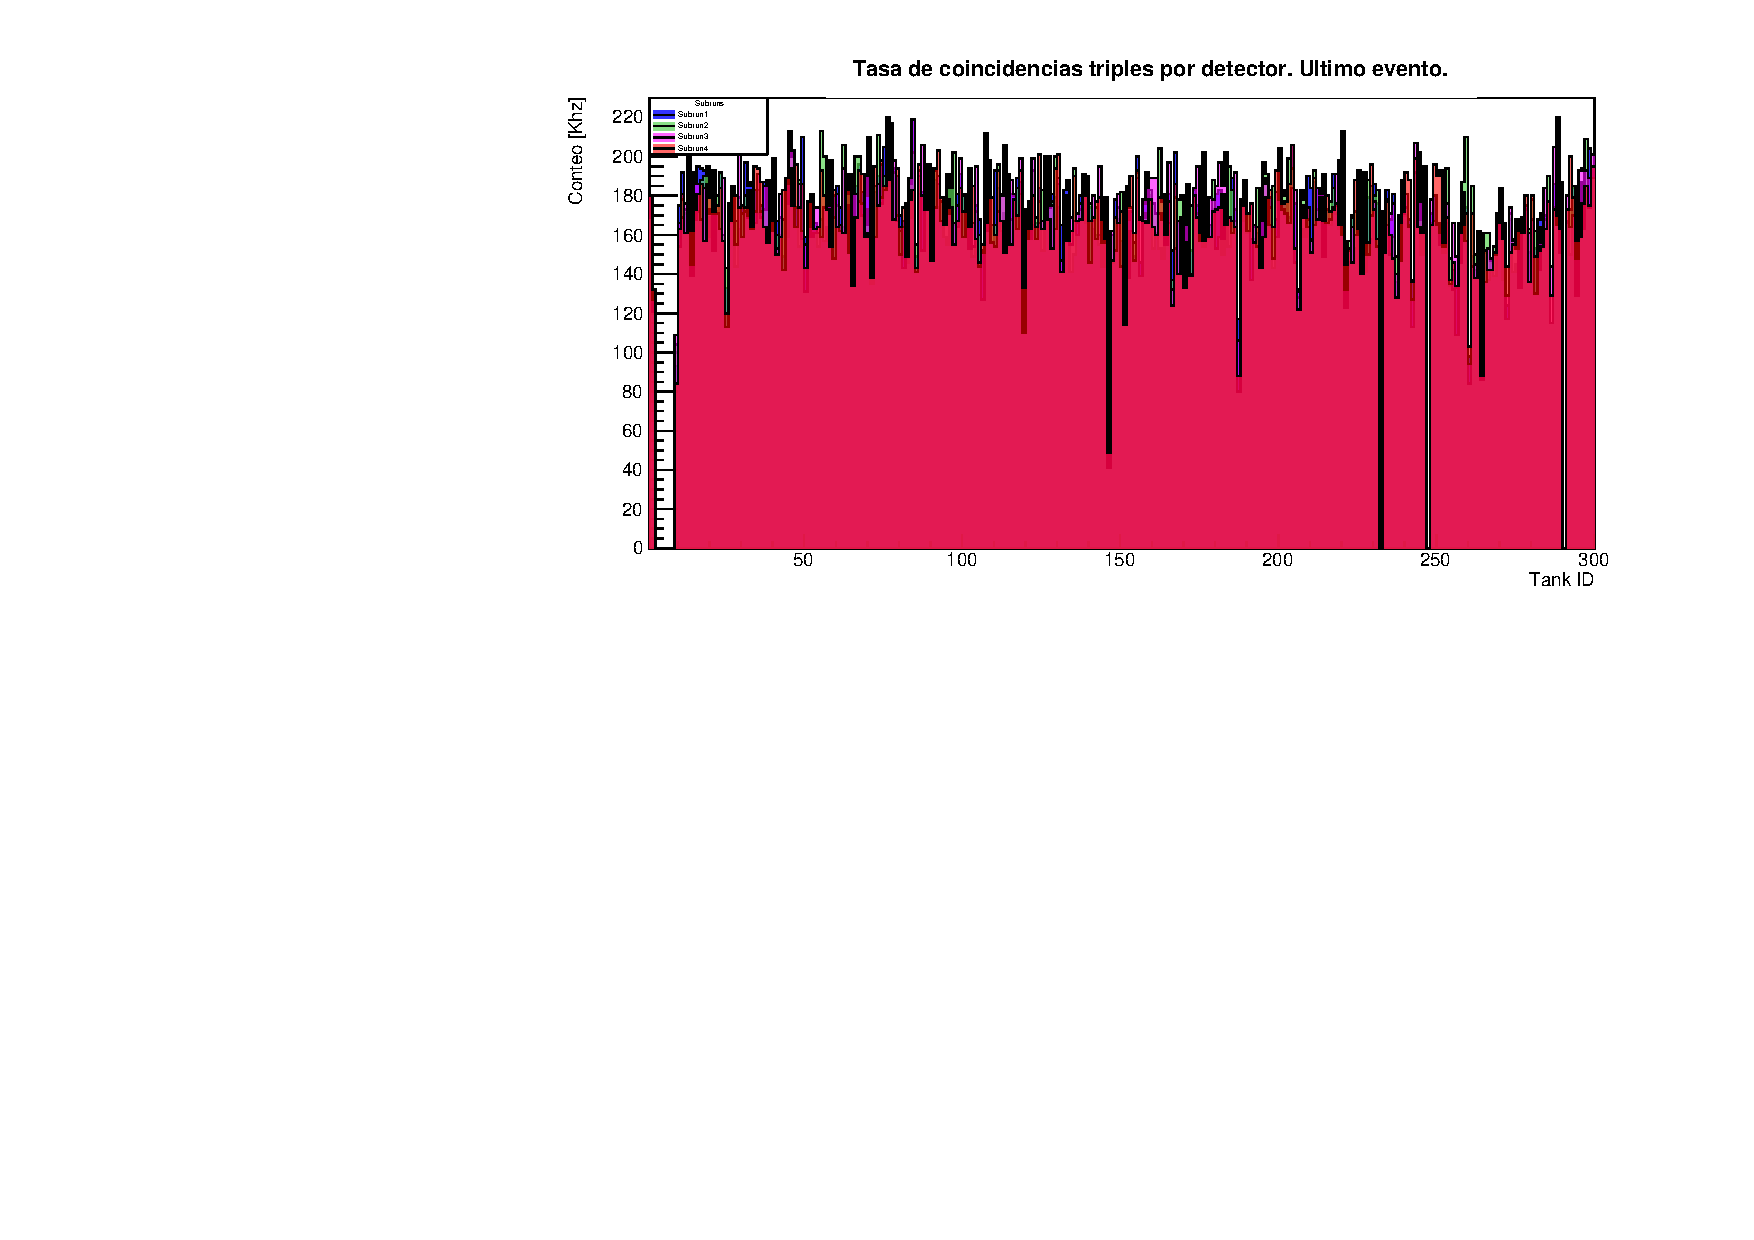
\includegraphics[width=0.9\textwidth]{../Figuras/CoinTriplesSubrunsUE.pdf}}

\subfloat[\centering Coincidencias cuádruples para diferentes subruns, último evento.]{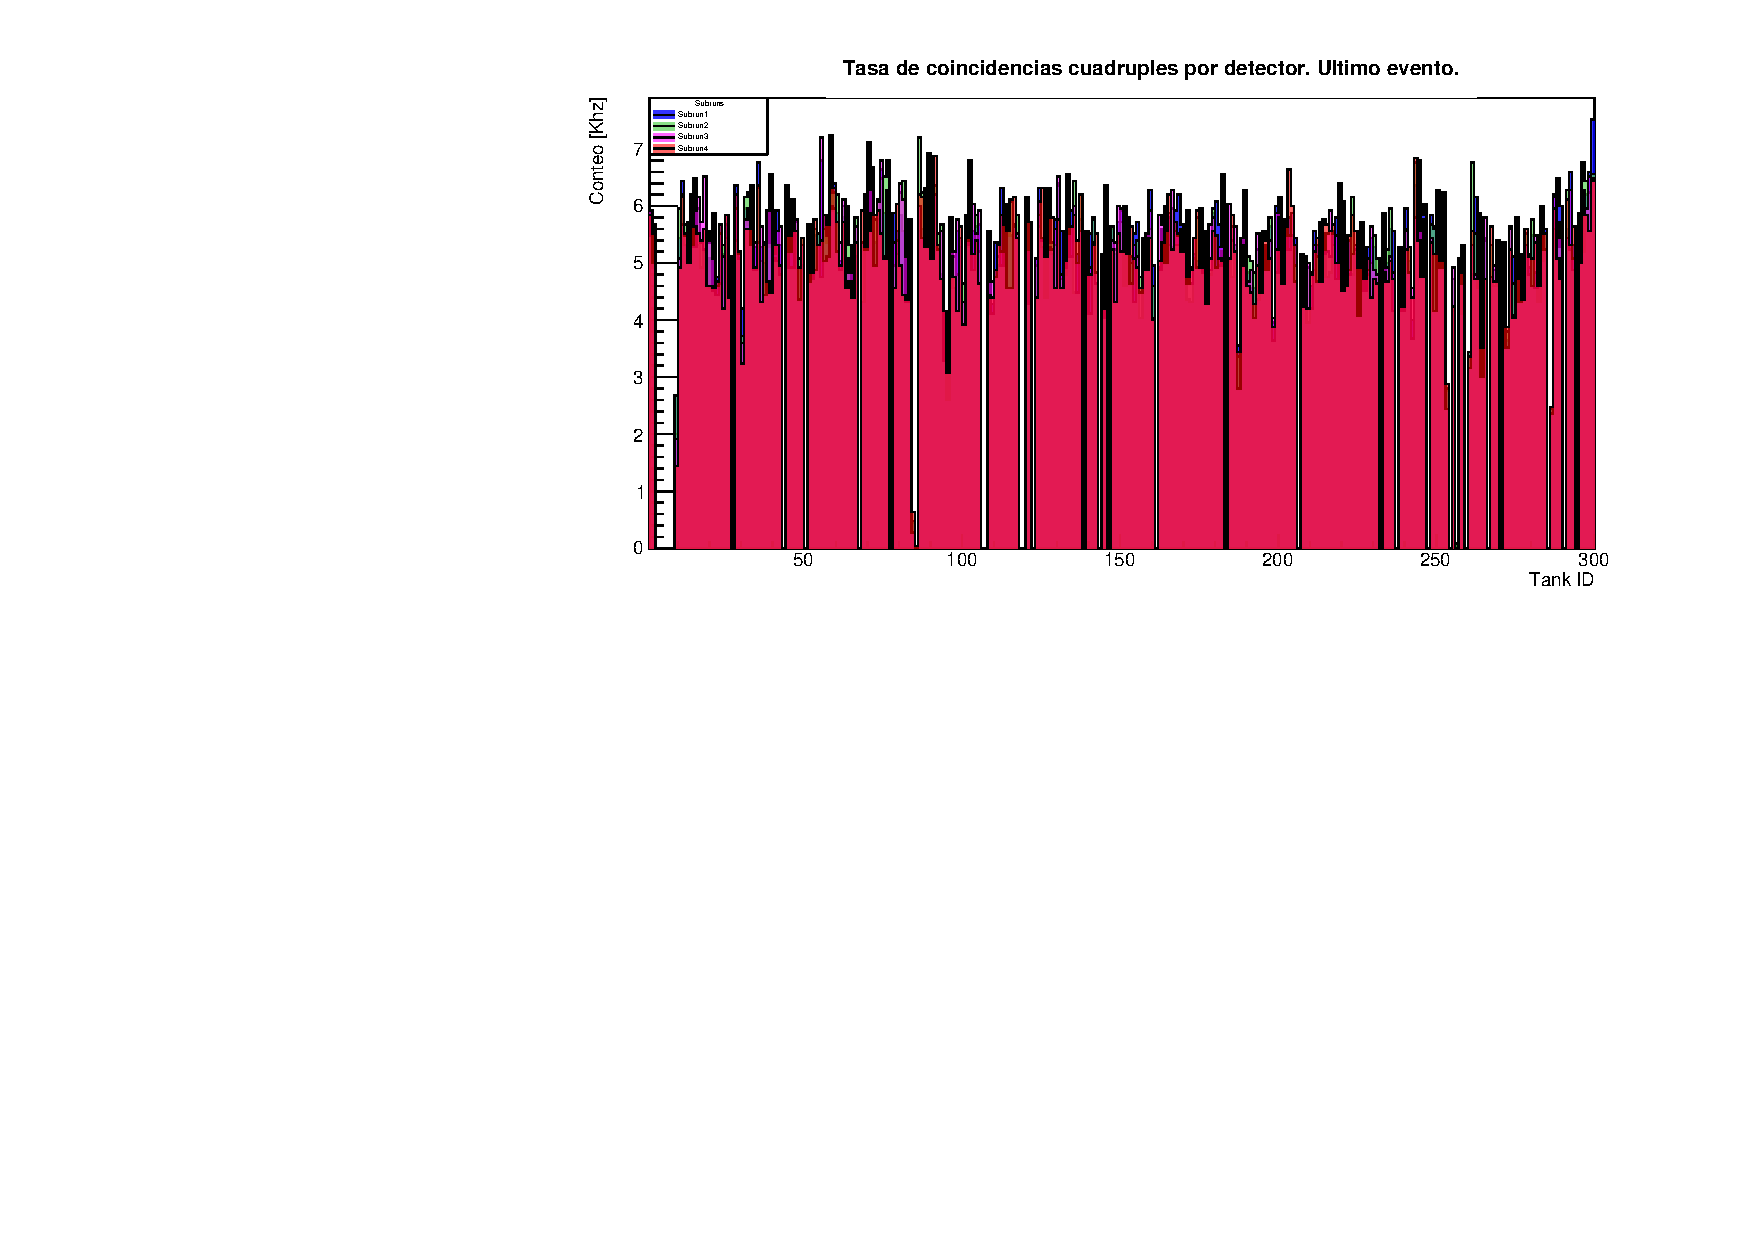
\includegraphics[width=0.9\textwidth]{../Figuras/CoinCuadruplesSubrunsUE.pdf}}
\caption{Tasas de conteo de coincidencias para el primer evento usando diferentes subruns. De arribo a abajo se van mostrando los resultados para coincidencias dobles, triples y cuádruples.}
\label{fig:Prob7-2}
\end{figure}

\textbf{Calcula la tasa de conteo de muones esperada en un detector de HAWC}

De acuerdo con los datos proporcionados en la clase, la intensidad del detector es $I=70\, \frac{1}{\textrm{m$^2$ $\cdot$ s$\cdot$ sr}}$. Considerando la geometría de la figura \ref{fig:detector}, observamos que el ángulo sólido de detección es \begin{equation}
\Omega = \frac{A}{h^2} = \frac{\pi (3.75\,\textrm{m})^2}{4.5\,\textrm{m}},
\end{equation}de esta forma, la frecuencia de detección de muones es \begin{equation}
f = I\cdot \Omega\cdot A \simeq 6.75\textrm{ kHz}.
\end{equation}Observemos que esta cantidad es del orden de magnitud de la tasa de conteo de las coincidencias triples y cuádruples que hemos mostrado en las figuras \ref{fig:Prob5-1} y \ref{fig:Prob5-2}.

\begin{figure}[H]
\centering
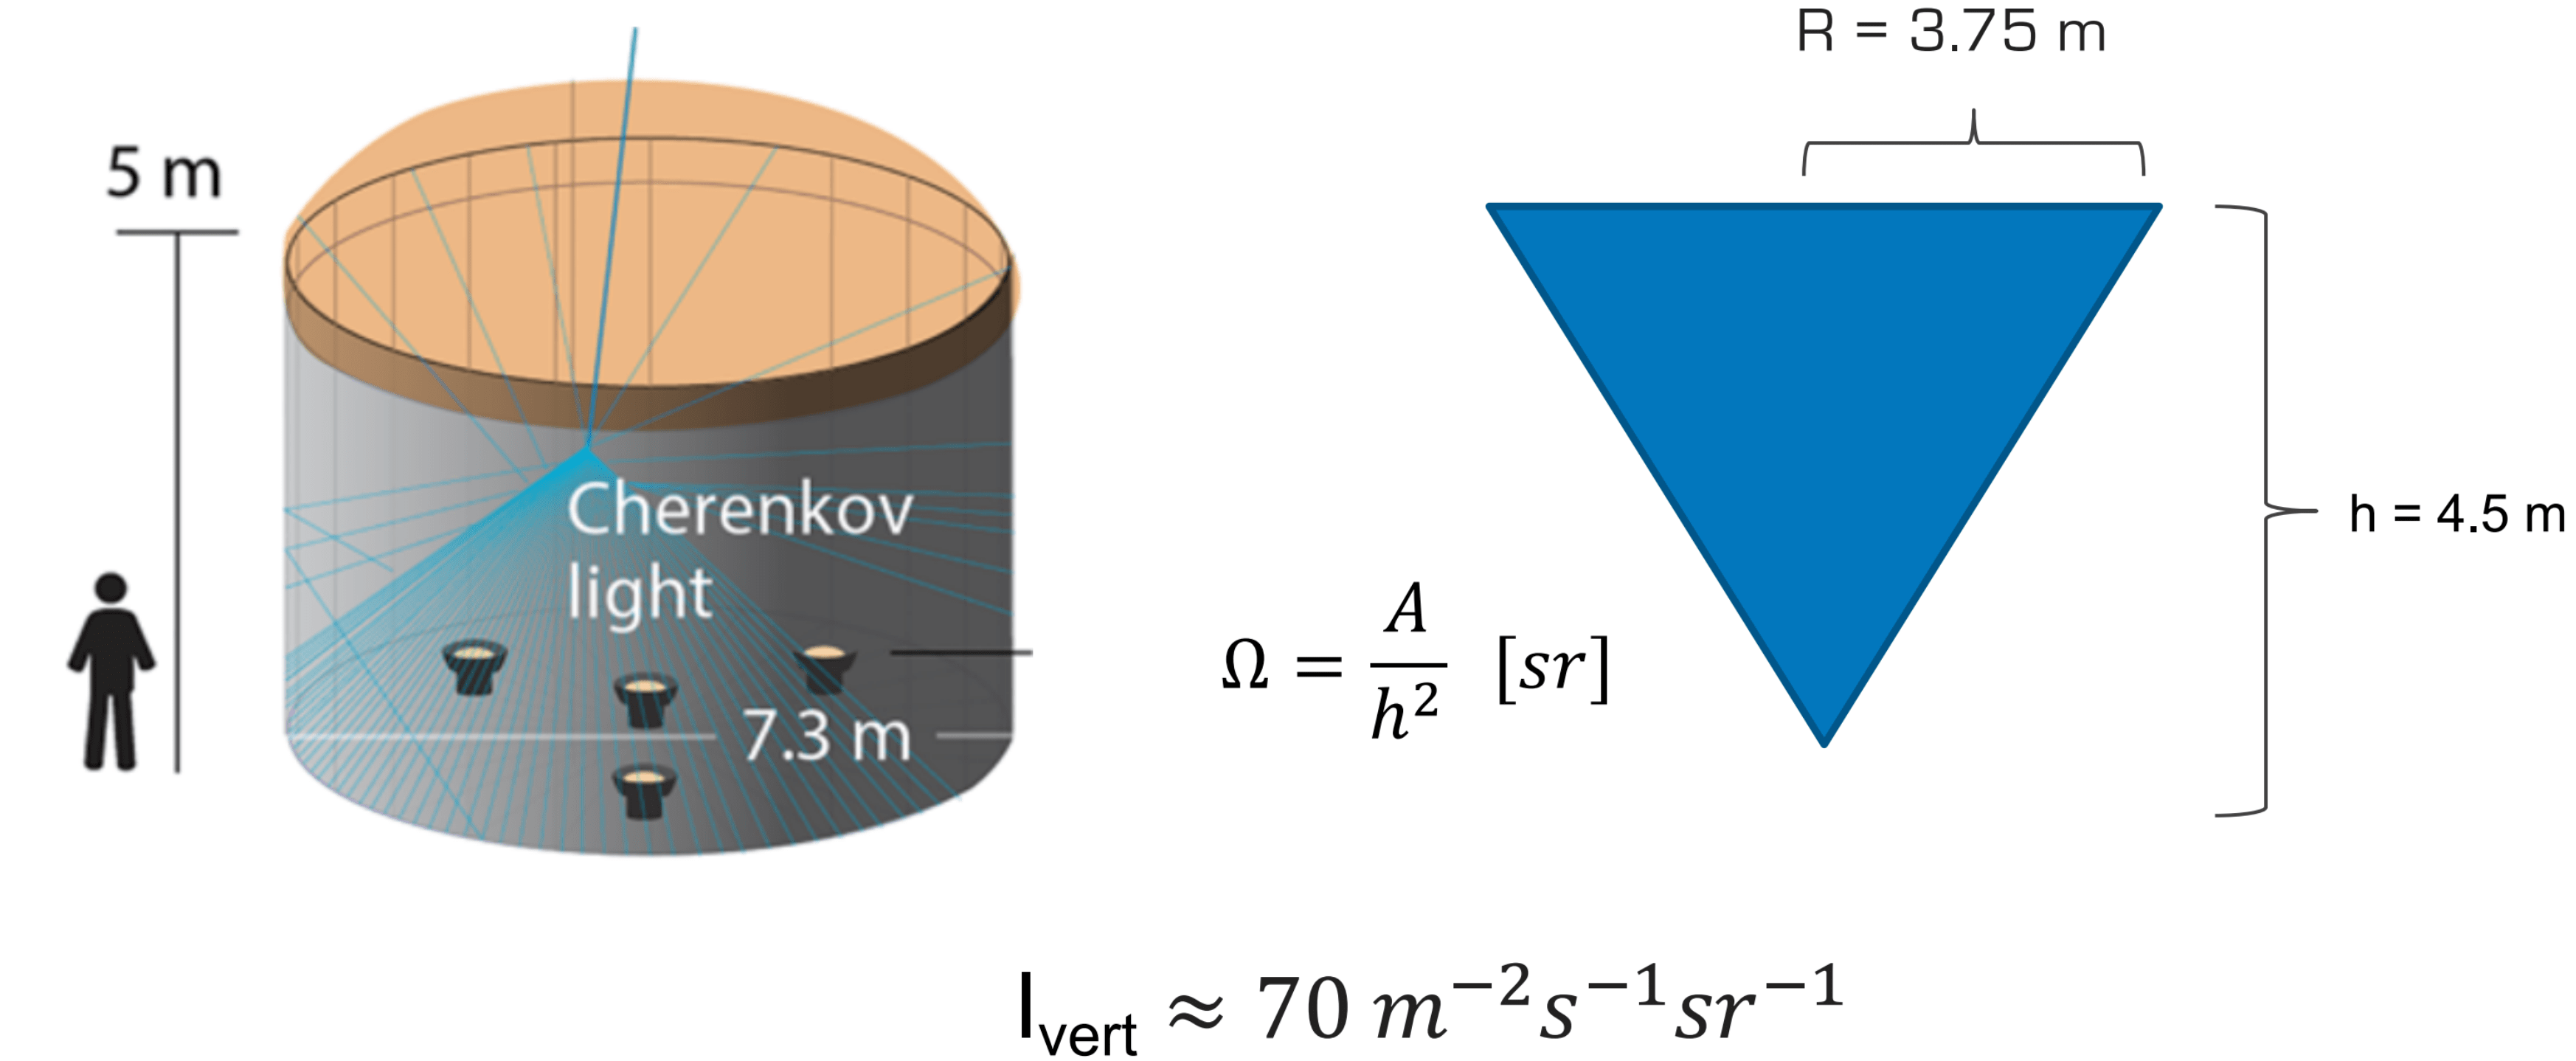
\includegraphics[width=0.8\textwidth]{../Figuras/detector.png}
\caption{Geometría del detector de HAWC. Imagen tomada de la presentación de la clase.}
\label{fig:detector}
\end{figure}


\end{document}